\documentclass[a4paper, 14pt]{article}
\usepackage[T2A]{fontenc}
\usepackage[utf8]{inputenc}
\usepackage[russian]{babel}
\usepackage{geometry}
\usepackage{array}
\usepackage{graphicx}
\usepackage{setspace}
\usepackage{siunitx}
\usepackage{caption}
\usepackage{titlesec}
\usepackage{indentfirst}
\usepackage{float}
\usepackage{array}
\usepackage{cellspace}
\usepackage{pgfplots}
\usepackage{pgfplotstable}
\usepackage{tocloft}
\usepackage{amsmath}
\usepackage{multicol}
\usepackage{minted}
\usepackage{tikz-timing}

\setlength{\cellspacetoplimit}{20pt}
\setlength{\cellspacebottomlimit}{20pt}

\onehalfspacing

\geometry{
  a4paper,
  left=30mm,
  right=20mm,
  top=20mm,
  bottom=20mm
}

\setlength{\parindent}{1.25cm}

\graphicspath{ {images/} }
\captionsetup[figure]{
  labelsep=period,
  justification=centering
}

\renewcommand{\figurename}{Рисунок}
\renewcommand{\contentsname}{Оглавление}

\titleformat{\section}[block]{\normalsize\bfseries}{\thesection}{1em}{}
\titleformat{\subsection}[block]{\normalsize\bfseries}{\thesubsection}{1em}{}
\titlespacing*{\section}{0pt}{\parskip}{-\parskip}
\titlespacing*{\subsection}{0pt}{\parskip}{-\parskip}

\renewcommand{\cftbeforetoctitleskip}{-30pt}
\renewcommand{\cftaftertoctitleskip}{-10pt}

\begin{document}

\begin{titlepage}
  \begin{center}
    \small
    \underline{
      \begin{minipage}{0.2\textwidth}
        \centering
        
\includegraphics[width=3cm]{BMSTU logo}
      \end{minipage}
      \hfill
      \begin{minipage}{0.8\textwidth}
        \begin{center}

          \textbf{Министерство науки и высшего образования Российской Федерации
            Федеральное государственное бюджетное образовательное учреждение высшего образования «Московский государственный технический университет имени Н.Э. Баумана национальный исследовательский университет»
          (МГТУ им. Н.Э. Баумана)}
        \end{center}
      \end{minipage}

    }

    \vspace{7cm}
    \Large
    \textbf{Модульное домашнее задание №2} \\
    \textbf{Вариант 12} \\
    Методы кодирования цифровых данных
    \\
    \vspace{5cm}
    \normalsize
    \begin{tabular}{p{8cm}p{6cm}}
      \textbf{Студент группы ИУ1-31Б} & Соин А. Д. \\
      & «15» мая 2026 г. \\
      & \\
      \textbf{Преподаватель} & Кузнецов М. А. \\
      & «\underline{\hspace{1.5cm}}»\underline{\hspace{2.5cm}}2025 г. \\
    \end{tabular}
    \vfill{\Large{Москва, 2026}}
  \end{center}
\end{titlepage}

\tableofcontents
\newpage

\section{Составление временных диаграм}

Задание по варианту

\begin{table}[H]
  \centering
  \begin{tabular}{|c|c|}
    \hline
    Вариант & Число \\ \hline
    12 & 46 \\ \hline
  \end{tabular}
\end{table}

Побитовое представление числа : $46_{10} = 00101110_2$

\subsection{RS-423}
Так как передача осуществляется от старшего бита к младшему: $ 01110100 $

Стартровый бит: $0 $.

Сообщение: $01110100$.

Стоповый бит: $1$.

Итоговое сообщение: $0011101001$

\begin{figure}[H]
  \begin{center}
    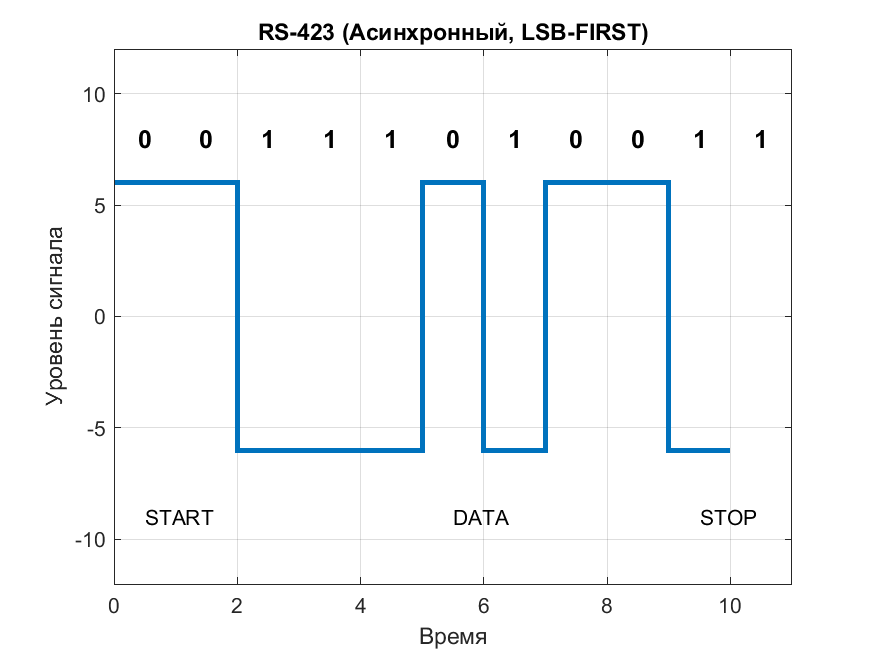
\includegraphics[width=0.6\textwidth]{rs423.png}
  \end{center}
\end{figure}

\subsection{RS-485}
В отличие от RS-423 является дифференциальным, т.е. у него два сигнальных провода (A – неинвертированный, B – инвертированный). Остальные параметры схемы передачи такие же, как у RS-423 (Idle, стартовый бит, передача и стоп-бит).

\begin{figure}[H]
  \begin{center}
    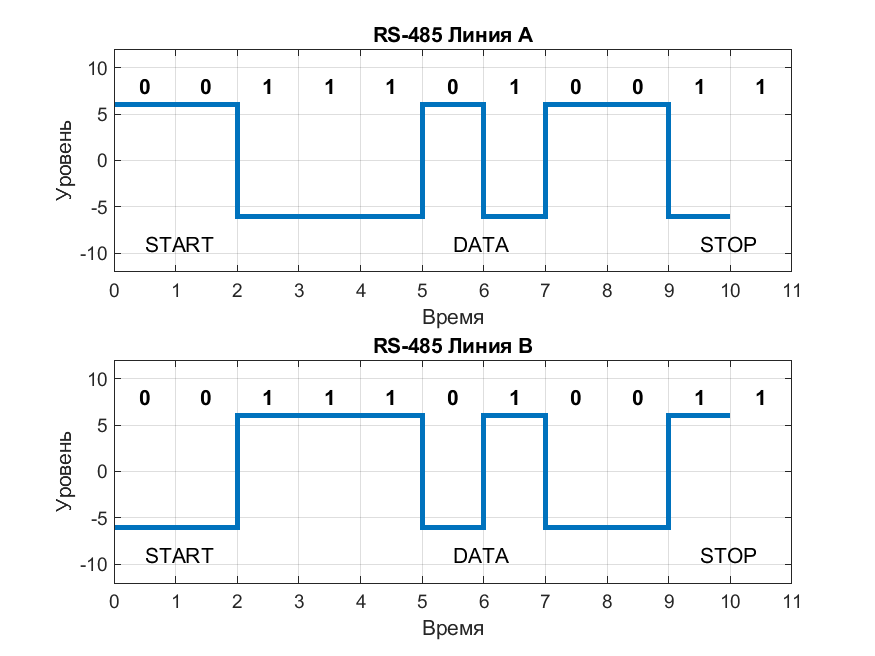
\includegraphics[width=0.6\textwidth]{rs485.png}
  \end{center}
\end{figure}

\subsection{SPI (CPOL = 0, CPHA = 1)}
Синхронный интерфейс, использующий 4 линии (SCLK, MOSI, MISO, SS).По линии SCK сигнал синхронизации CPOL = 0 значит, что в покое уровень 0. По линии MOSI передачи данных от ведущего к ведомому CPHA = 1 значит, что смена уровня происходит по переднему фронту синхронизации, а выборка данных – по заднему фронту. Передача ведётся от старшего бита к младшему (MSB First), т.е. для числа 46, следовательно сообщение: $00101110$

\begin{figure}[H]
  \begin{center}
    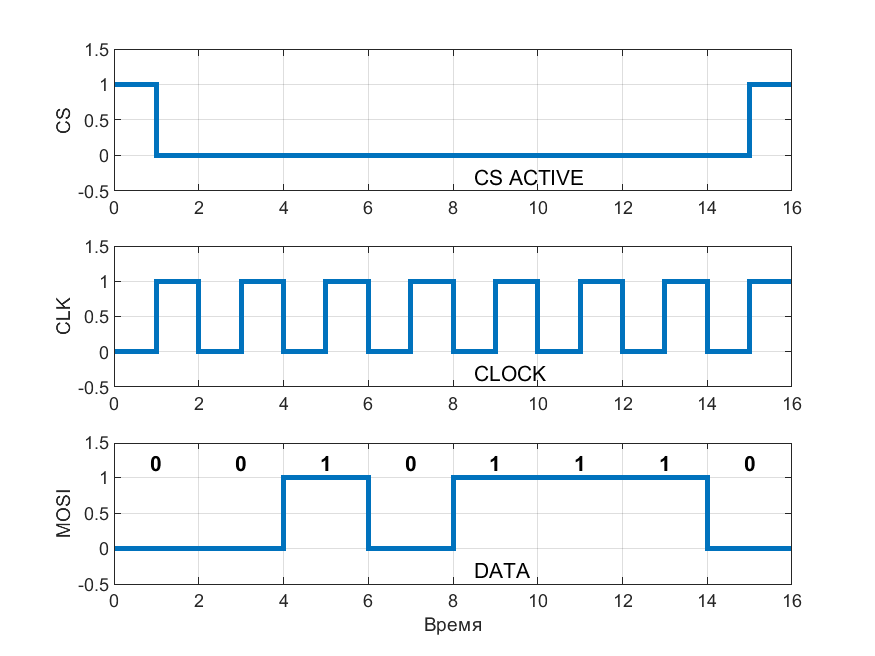
\includegraphics[width=0.6\textwidth]{spi.png}
  \end{center}
\end{figure}

\subsection{I2C (адрес 0x14)}
Последовательная ассиметричная шина с линиями SDA и SCL и системой переадресации. Покой - высокий уровень.Старт-бит – переход SDA из 1 в 0 при высоком уровне SCL.
Далее передаётся адрес (7 бит), в нашем случае 0x14 ($0010100_2$) (MSB First).
Затем идёт R/W бит (в нашем случае запись, поэтому 0).
ACK девятым тактом переводит линию SDA в 0.
Далее идёт информация в формате MSB First.
Затем снова ACK для подтверждения. Стоп-бит – переход SDA из 0 в 1 при высоком SCL.

\begin{figure}[H]
  \begin{center}
    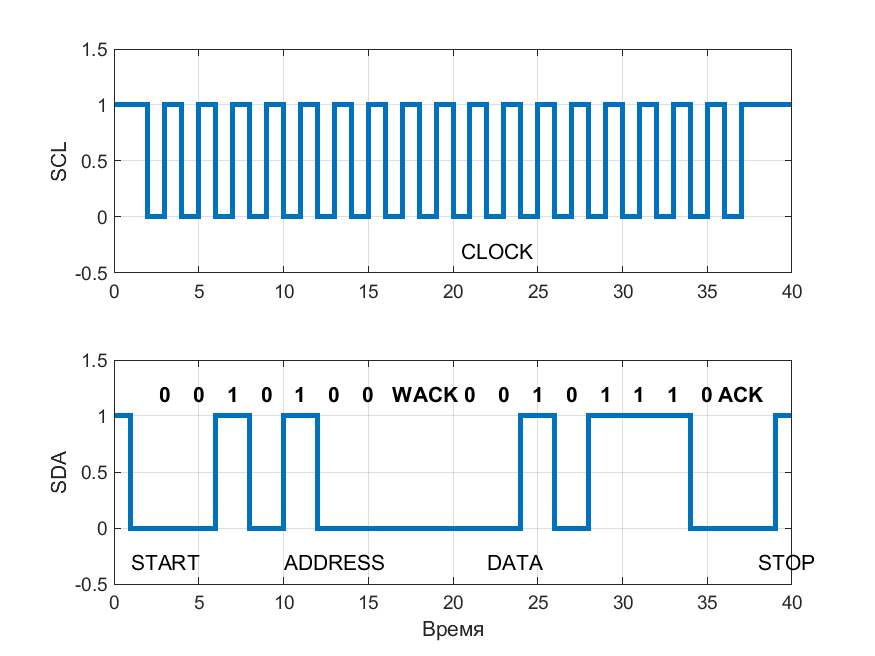
\includegraphics[width=0.6\textwidth]{i2c.png}
  \end{center}
\end{figure}

\subsection{USB 2.0}

Данные передаются по дифференциальной паре D+ и D- кодированием NRZI. Верхний уровень напряжения – 1, нижний – 0. Передача идёт  в формате LSB First.

\begin{figure}[H]
  \begin{center}
    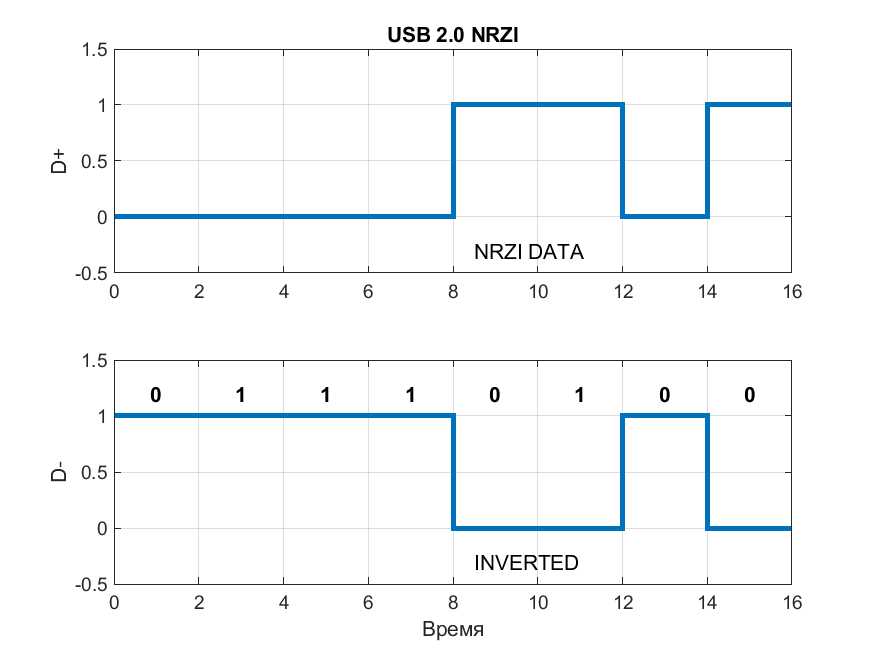
\includegraphics[width=0.6\textwidth]{usb20.png}
  \end{center}
\end{figure}

\subsection{1-Wire (адрес устройства 0x14)}

Представляет собой один провод для питания и данных.
Сначала идёт сброс линии мастером к 0 на длительное время на 480 мкс.
Затем мастер отпускает линию, и ведомый через небольшую паузу сам прижимает
линию к 0 на 60-240 мкс в виде импульса присутствия.
Далее мастер передаёт команду Match ROM (0x55) в LSB First виде: $10101010$.
Затем 8-битный адрес в LSB First виде, в нашем случае 0x14: $00101000$.
Затем идут данные также в LSB First.
0 значит широкий провал, почти на всю длительность тайм-слота (60-120 мкс);
1 – короткий провал (8-15 мкс).

\begin{figure}[H]
  \begin{center}
    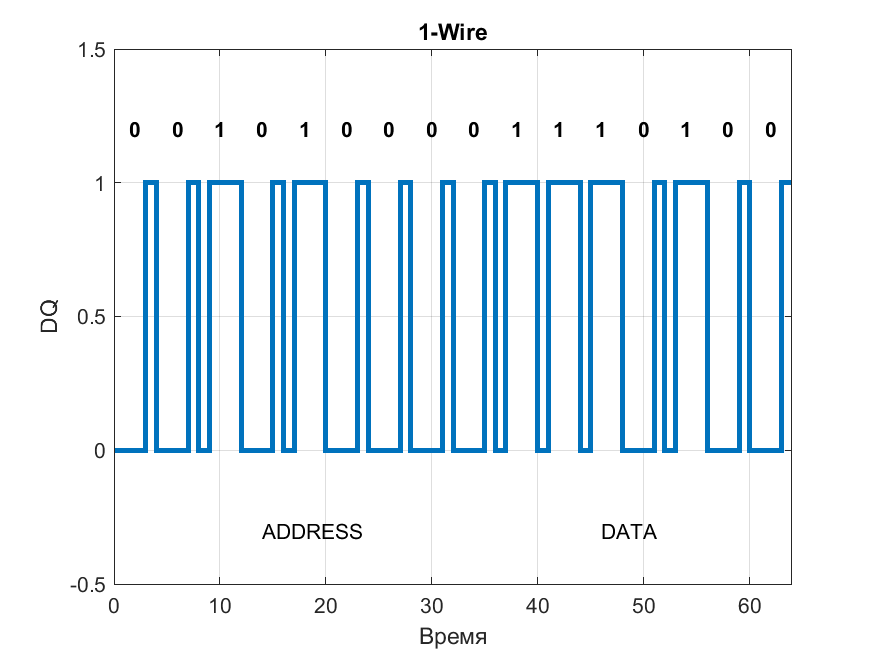
\includegraphics[width=0.6\textwidth]{1wire.png}
  \end{center}
\end{figure}

\section{Получение разных представлений числа}

Так как вариант является четным работа будет идти с числом 46.

\subsection{Беззнаковое двухбайтное целое}

В таком представлении имеем $46_{10} = 0000000000101110_2$

\subsection{Знаковое двухбайтное целое}

При записи числа в знаковом виде старший бит отвечает за знак:
если число отрицательное, этот бит равен 1, иначе – 0.
В нашем случае число $+46_10$ является положительным,
поэтому старший бит будет нулевым.
Тогда в виде знакового двухбайтного целого получим: $$0 000000000101110_2$$

\section{Получение дробного числа в формате с плавающей точкой одинарной точности}

Так как вариант является четным работа будет идти с числом $46/25 = 1.84$.

Представление числа в формате одинарной точности:$$ V = (-1)^S \cdot C \cdot b^Q $$
, где S - первый бит, b - основание, Q - порядок, C - мантиса.

Бит знака: $S = 0$.

Целая часть: $1_{10}  = 1_2$.

Дробная часть:
\begin{table}[H]
  \center
  \begin{tabular}{|c|c|c|}
    \hline
    Порядок & Дробная часть & Бит \\ \hline
    1 & 0.84 & 1\\ \hline
    2 & 0.68 & 1\\ \hline
    3 & 0.36 & 0\\ \hline
    4 & 0.72 & 1\\ \hline
    5 & 0.44 & 0\\ \hline
    6 & 0.88 & 1\\ \hline
    7 & 0.76 & 1\\ \hline
    8 & 0.52 & 1\\ \hline
    9 & 0.04 & 0\\ \hline
    10 & 0.08 & 0\\ \hline
    11 & 0.16 & 0\\ \hline
    12 & 0.32 & 0\\ \hline
    13 & 0.64 & 1\\ \hline
    14 & 0.28 & 0\\ \hline
    15 & 0.56 & 1\\ \hline
    16 & 0.12 & 0\\ \hline
    17 & 0.24 & 0\\ \hline
    18 & 0.48 & 0\\ \hline
    19 & 0.96 & 1\\ \hline
    20 & 0.92 & 1\\ \hline
    21 & 0.84 & 1\\ \hline
    22 & 0.68 & 1\\ \hline
    23 & 0.36 & 0\\ \hline
  \end{tabular}
\end{table}

Таким образом $1.84_{10} = 1.11010111000010100011110_2$.
Смещение $127_{10} = 01111111$.
Мантисса $11010111000010100011110$.

Тогда число имеет следующий вид $0 01111111 11010111000010100011110$

Проведем оьбратную проверку:$$ +1 \cdot 2^{127-127} \cdot 1.83999991416931152343750 = 1.83999991416931152343750$$

Число близко к исходному, но не равно ему, так как 0.84 нельзя точно представить в двоичной форме.
\end{document}